\documentclass{beamer}
\usepackage{amsmath}
\usepackage[english]{babel} %set language; note: after changing this, you need to delete all auxiliary files to recompile
\usepackage[utf8]{inputenc} %define file encoding; latin1 is the other often used option
\usepackage{csquotes} % provides context sensitive quotation facilities
\usepackage{graphicx} %allows for inserting figures
\usepackage{booktabs} % for table formatting without vertical lines
\usepackage{textcomp} % allow for example using the Euro sign with \texteuro
\usepackage{stackengine}
\usepackage{wasysym}
\usepackage{tikzsymbols}
\usepackage{textcomp}
% ELIMINAR COMANDOS DE NAVEGACION%%%%%%%%%%%
\setbeamertemplate{navigation symbols}

%\newcommand{\bubblethis}[2]{
 %       \tikz[remember picture,baseline]{\node[anchor=base,inner sep=0,outer sep=0]%
 %       (#1) {\underline{#1}};\node[overlay,cloud callout,callout relative pointer={(0.2cm,-0.7cm)},%
 %       aspect=2.5,fill=yellow!90] at ($(#1.north)+(-0.5cm,1.6cm)$) {#2};}%
 %   }%
%\tikzset{face/.style={shape=circle,minimum size=4ex,shading=radial,outer sep=0pt,
 %       inner color=white!50!yellow,outer color= yellow!70!orange}}

%% Some commands to make the code easier
\newcommand{\emoticon}[1][]{%
  \node[face,#1] (emoticon) {};
  %% The eyes are fixed.
  \draw[fill=white] (-1ex,0ex) ..controls (-0.5ex,0.2ex)and(0.5ex,0.2ex)..
        (1ex,0.0ex) ..controls ( 1.5ex,1.5ex)and( 0.2ex,1.7ex)..
        (0ex,0.4ex) ..controls (-0.2ex,1.7ex)and(-1.5ex,1.5ex)..
        (-1ex,0ex)--cycle;}
\newcommand{\pupils}{
  %% standard pupils
  \fill[shift={(0.5ex,0.5ex)},rotate=80] 
       (0,0) ellipse (0.3ex and 0.15ex);
  \fill[shift={(-0.5ex,0.5ex)},rotate=100] 
       (0,0) ellipse (0.3ex and 0.15ex);}

\newcommand{\emoticonname}[1]{
  \node[below=1ex of emoticon,font=\footnotesize,
        minimum width=4cm]{#1};}
\usepackage{scalerel}
\usetikzlibrary{positioning}
\usepackage{xcolor,amssymb}
\newcommand\dangersignb[1][2ex]{%
  \scaleto{\stackengine{0.3pt}{\scalebox{1.1}[.9]{%
  \color{red}$\blacktriangle$}}{\tiny\bfseries !}{O}{c}{F}{F}{L}}{#1}%
}
\newcommand\dangersignw[1][2ex]{%
  \scaleto{\stackengine{0.3pt}{\scalebox{1.1}[.9]{%
  \color{red}$\blacktriangle$}}{\color{white}\tiny\bfseries !}{O}{c}{F}{F}{L}}{#1}%
}
\usepackage{fontawesome} % Social Icons
\usepackage{epstopdf} % allow embedding eps-figures
\usepackage{tikz} % allows drawing figures
\usepackage{amsmath,amssymb,amsthm} %advanced math facilities
\usepackage{lmodern} %uses font that support italic and bold at the same time
\usepackage{hyperref}
\usepackage{tikz}
\hypersetup{
    colorlinks=true,
    linkcolor=blue,
    filecolor=magenta,      
    urlcolor=blue,
}
\usepackage{tcolorbox}
%add citation management using BibLaTeX
\usepackage[citestyle=authoryear-comp, %define style for citations
    bibstyle=authoryear-comp, %define style for bibliography
    maxbibnames=10, %maximum number of authors displayed in bibliography
    minbibnames=1, %minimum number of authors displayed in bibliography
    maxcitenames=3, %maximum number of authors displayed in citations before using et al.
    minnames=1, %maximum number of authors displayed in citations before using et al.
    datezeros=false, % do not print dates with leading zeros
    date=long, %use long formats for dates
    isbn=false,% show no ISBNs in bibliography (applies only if not a mandatory field)
    url=false,% show no urls in bibliography (applies only if not a mandatory field)
    doi=false, % show no dois in bibliography (applies only if not a mandatory field)
    eprint=false, %show no eprint-field in bibliography (applies only if not a mandatory field)
    backend=biber %use biber as the backend; backend=bibtex is less powerful, but easier to install
    ]{biblatex}
\addbibresource{../mybibfile.bib} %define bib-file located one folder higher


\usefonttheme[onlymath]{serif} %set math font to serif ones

\definecolor{beamerblue}{rgb}{0.2,0.2,0.7} %define beamerblue color for later use

%%% defines highlight command to set text blue
\newcommand{\highlight}[1]{{\color{blue}{#1}}}


%%%%%%% commands defining backup slides so that frame numbering is correct

\newcommand{\backupbegin}{
   \newcounter{framenumberappendix}
   \setcounter{framenumberappendix}{\value{framenumber}}
}
\newcommand{\backupend}{
   \addtocounter{framenumberappendix}{-\value{framenumber}}
   \addtocounter{framenumber}{\value{framenumberappendix}}
}

%%%% end of defining backup slides

%Specify figure caption, see also http://tex.stackexchange.com/questions/155738/caption-package-not-working-with-beamer
\setbeamertemplate{caption}{\insertcaption} %redefines caption to remove label "Figure".
%\setbeamerfont{caption}{size=\scriptsize,shape=\itshape,series=\bfseries} %sets figure  caption bold and italic and makes it smaller


\usetheme{Boadilla}

%set options of hyperref package
\hypersetup{
    bookmarksnumbered=true, %put section numbers in bookmarks
    naturalnames=true, %use LATEX-computed names for links
    citebordercolor={1 1 1}, %color of border around cites, here: white, i.e. invisible
    linkbordercolor={1 1 1}, %color of border around links, here: white, i.e. invisible
    colorlinks=true, %color links
    anchorcolor=black, %set color of anchors
    linkcolor=beamerblue, %set link color to beamer blue
    citecolor=blue, %set cite color to beamer blue
    pdfpagemode=UseThumbs, %set default mode of PDF display
    breaklinks=true, %break long links
    pdfstartpage=1 %start at first page
    }


% --------------------
% Overall information
% --------------------
\title[Economía I]{Economía I \vspace{4mm}
\\ Magistral 11: Elasticidad}
\date{}
\author[Ertola Navajas y Fariña]{Ertola Navajas y Fariña}
\vspace{0.4cm}
\institute[]{Universidad de San Andrés} 

\begin{document}

\begin{frame}
\titlepage
\centering

\includegraphics[scale=0.2]{Slides Principios de Economia/Figures/logoUDESA.jpg} 
\end{frame}

\begin{frame}
\frametitle{Y si aumentó el precio...}
\centering
\href{https://econ.video/2017/08/02/the-simpsons-bart-gets-an-elephant/}{\includegraphics[scale=0.4]{Slides Principios de Economia/Figures/Homeroyelefante.png}}
\end{frame}

%\begin{frame}{Elasticidad precio de rutas áereas}
%\centering
%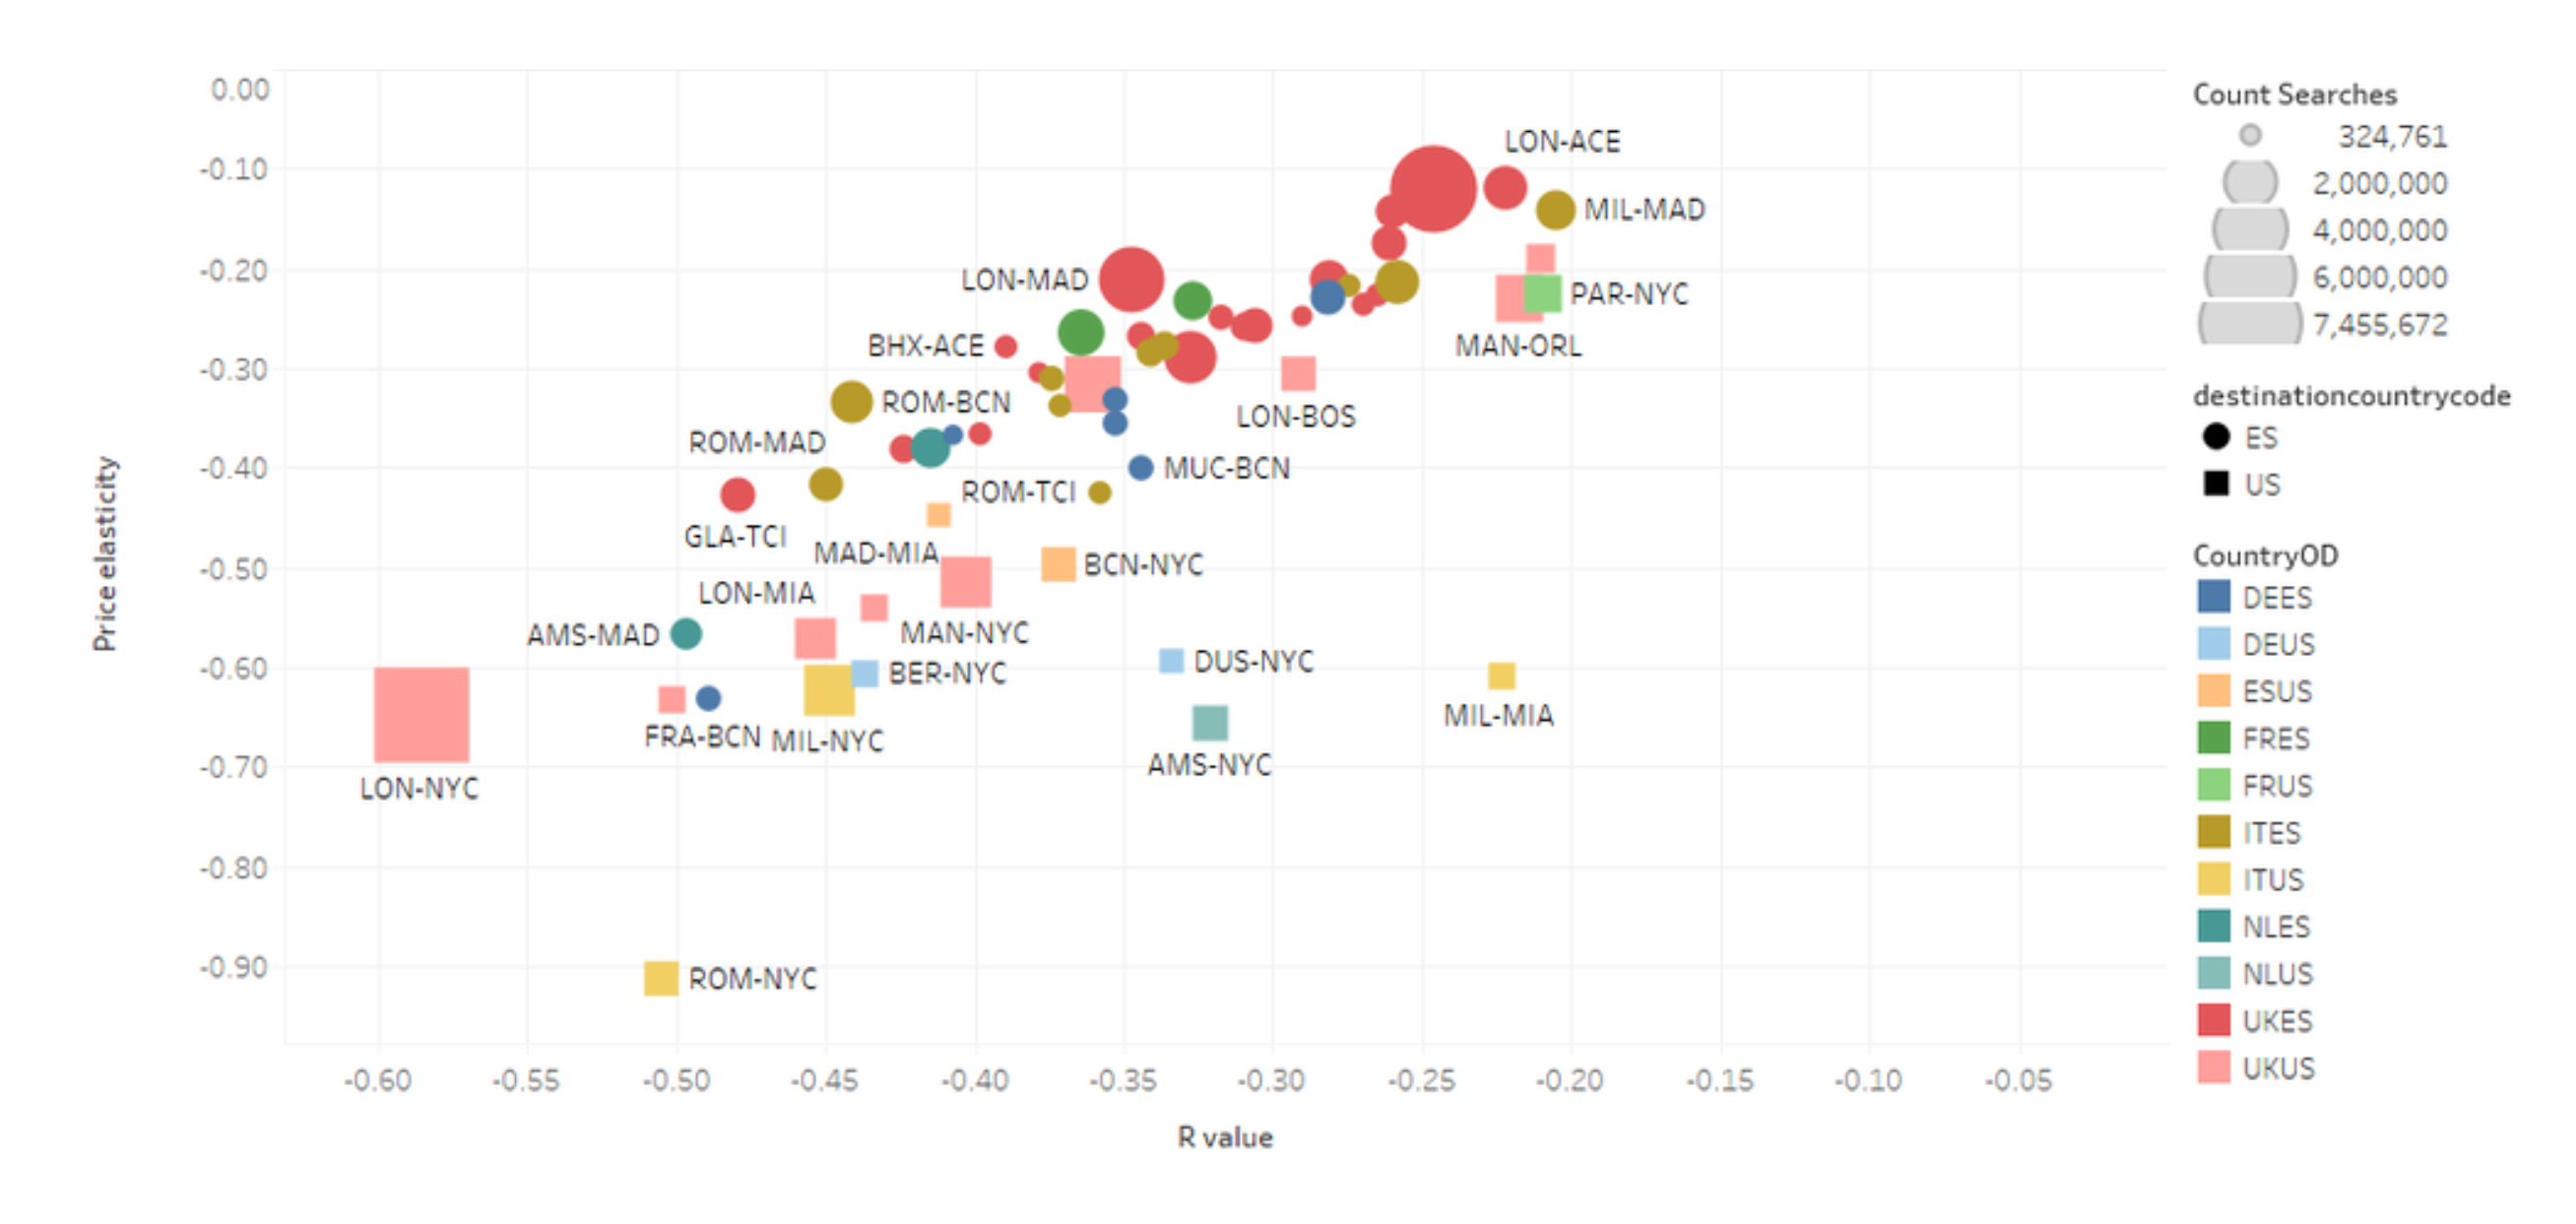
\includegraphics[scale=0.55]{Slides Principios de Economia/Figures/ElasticidadVuelos.png}
%\end{frame}

\begin{frame}
\frametitle{Sensibilidad de la demanda}
\begin{itemize}
    \item La pendiente de la curva de demanda tiene información relevante para las empresas\vspace{2mm}
    \begin{itemize}
        \item La pendiente muestra la relación costo-beneficio que la firma enfrenta entre precio y cantidad.\vspace{4mm}
     \end{itemize}
    \item ¿Nos ayuda a pensar qué tan sensible es la demanda ante cambios en los precios?\vspace{2mm}
    \begin{itemize}
        \item En parte, si, pero para pensar en esto usamos el concepto de \textbf{elasticidad-precio}: \\\vspace{2mm}
      \item Intuitivamente, se refiere al grado de reacción de los consumidores a cambios en el precio del producto 
    \end{itemize}
    \end{itemize}
\end{frame}

\begin{frame}
\frametitle{Elasticidad precio de la demanda}
\begin{itemize}
    \item A diferencia de la pendiente, la elasticidad precio mira cambios porcentuales:
    \begin{center}
    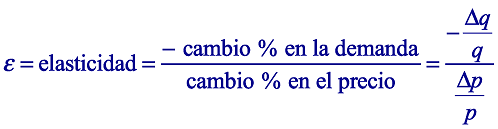
\includegraphics[scale=0.7]{Slides Principios de Economia/Figures/Tema_06.43_elasticidadformula.png}
    \end{center}
    \end{itemize}
\end{frame}

\begin{frame}
\frametitle{Elasticidad precio de la demanda}
\begin{itemize}
    \item Medida de sensibilidad: ¿cuál es el cambio \% en la cantidad demandada ante un cambio de 1\% en el precio? \\\vspace{2mm}
    \begin{itemize}
        \item Como la demanda cae ante un aumento en el precio, se suele cambiar el signo para que la relación nos de positiva (esto facilita la interpretación)\vspace{4mm}
    \end{itemize}
    \item ¿Qué tan elástica? \\\vspace{2mm}
    - Si $e > 1$ decimos que la demanda es elástica \\
    - Si $e = 1$ decimos que la demanda es unitaria \\
    - Si $e < 1$ decimos que la demanda es inelástica
    \end{itemize}
\end{frame}

\begin{frame}
\frametitle{Determinantes de la elasticidad precio de la demanda}
\begin{itemize}
    \item Disponibilidad de sustitutos cercanos: bienes con sustitutos cercanos tienden a tener demandas más elásticas.\vspace{4mm}
 \item Necesidades vs Lujos: necesidades tienden a tener demandas inelásticas, mientras que los lujos demandas elásticas.\vspace{4mm}
\item Definición de mercado: Helado. Helado bombon escoces.\vspace{4mm}
\item Horizonte de tiempo: Gasolina. Cae poco la cantidad demandada en el CP y más en el LP
    \end{itemize}
\end{frame}

\begin{frame}
\frametitle{Elasticidad y pendiente}
\begin{itemize}
    \item Ambos conceptos están relacionados
    \begin{center}
    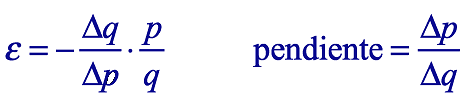
\includegraphics[scale=0.5]{Slides Principios de Economia/Figures/Tema_06.44_elasticidadpendiente.png}
    \end{center}
        \begin{itemize}
        \item La pendiente forma parte del concepto de elasticidad.\vspace{2mm}
        \item Una curva de demanda muy empinada es relativamente inelástica, y una bastante plana es elástica.\vspace{4mm}
        \end{itemize}
    \item ¡Pero no son lo mismo!\vspace{2mm}
        \begin{itemize}
            \item Notar que la elasticidad puede cambiar a medida que nos movemos a lo largo de la curva de demanda, aun si la pendiente no lo hace.\vspace{2mm}
            \item ¡Y viceversa!
        \end{itemize}
    \end{itemize}
\end{frame}

\begin{frame}
\frametitle{Elasticidad constante}
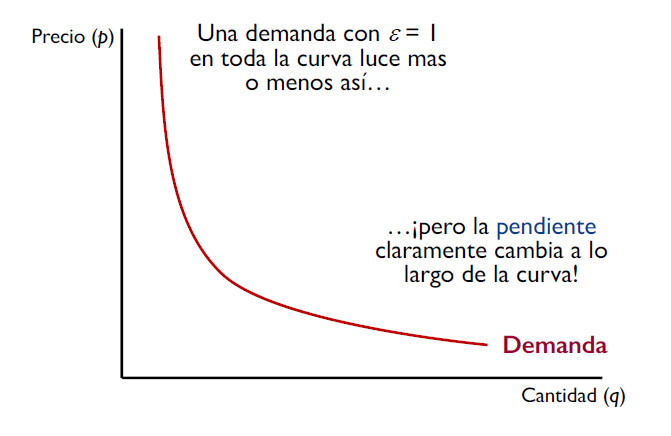
\includegraphics[scale=0.6]{Slides Principios de Economia/Figures/Tema_06.45_elasticidad.png}
\end{frame}

\begin{frame}
\frametitle{Pendiente constante}
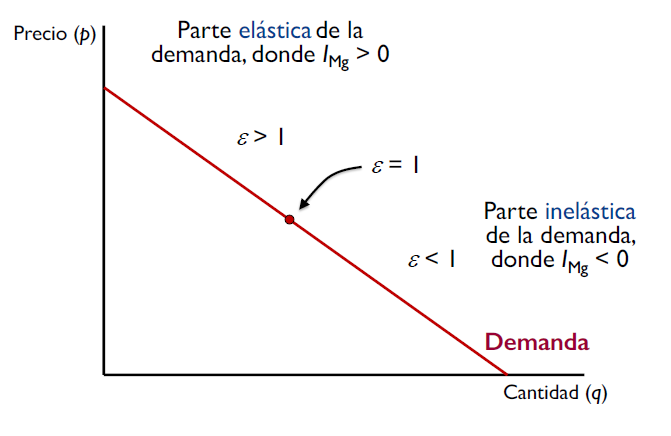
\includegraphics[scale=0.6]{Slides Principios de Economia/Figures/Tema_06.46_elasticidad2.png}
\end{frame}

\begin{frame}
\frametitle{¿Cómo son los excedentes con una demanda elástica?}
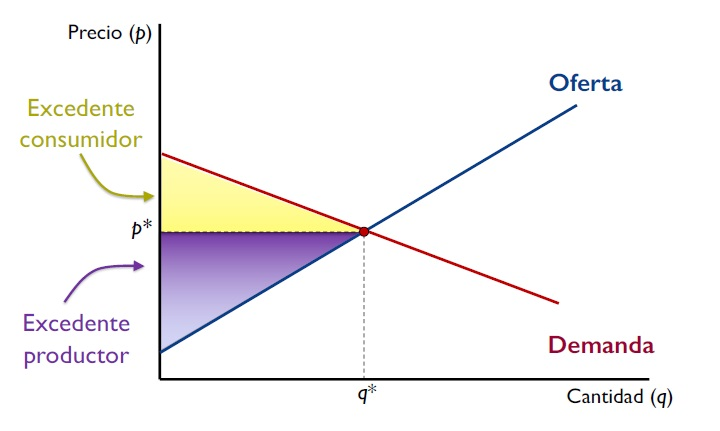
\includegraphics[scale=0.6]{Slides Principios de Economia/Figures/Tema_07.24_equilibrioyexcedente2.jpg}
\end{frame}

\begin{frame}
\frametitle{¿Cómo son los excedentes con una demanda inelástica?}
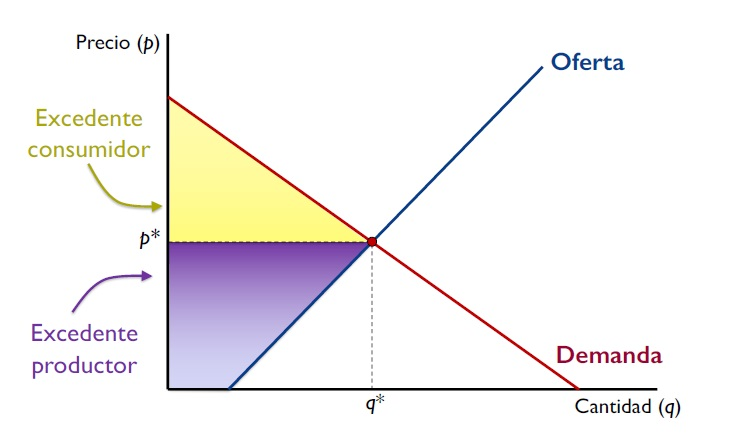
\includegraphics[scale=0.6]{Slides Principios de Economia/Figures/Tema_07.25_equilibrioyexcedente3.jpg}
\end{frame}

\begin{frame}
\frametitle{¿Cómo son los excedentes con una oferta elástica?}
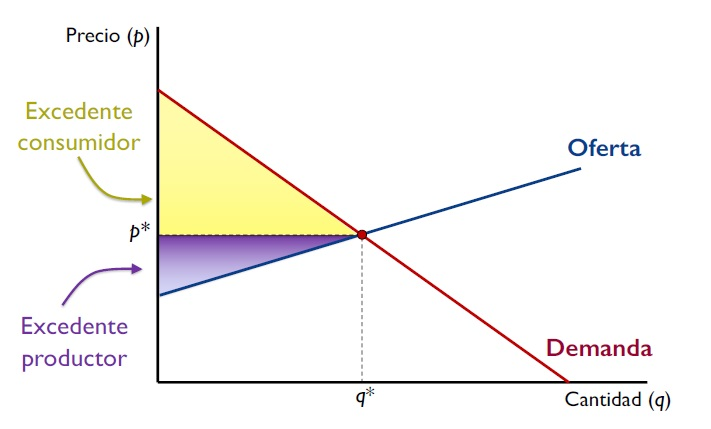
\includegraphics[scale=0.6]{Slides Principios de Economia/Figures/Tema_07.26_equilibrioyexcedente4.jpg}
\end{frame}

\begin{frame}
\frametitle{¿Cómo son los excedentes con una oferta inelástica?}
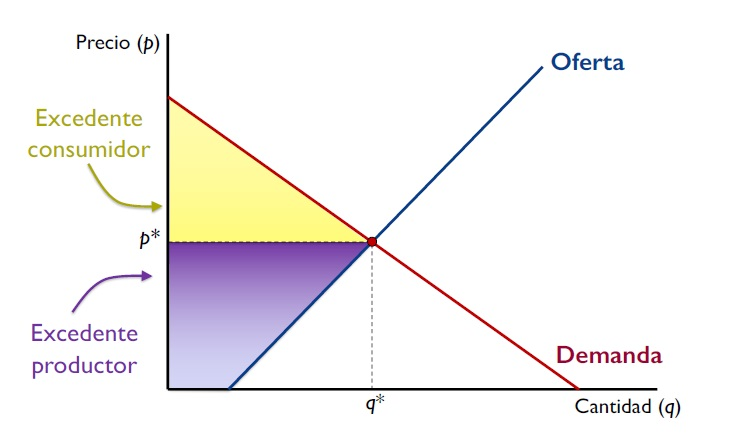
\includegraphics[scale=0.55]{Slides Principios de Economia/Figures/Tema_07.25_equilibrioyexcedente3.jpg}
\end{frame}

\begin{frame}
\frametitle{Ingreso total (pxq) y elasticidad}
\begin{itemize}
    \item El impacto de un cambio de precio en los ingresos totales, depende de la elasticidad de la demanda.
    \item Si la demanda es inelástica un incremento en el precio provoca un decremento en la cantidad demandada proporcionalmente más pequeño, por lo cual los ingresos totales se incrementan.
    \item Si la curva de la demanda es elástica, un incremento en el precio provoca una disminución en la cantidad demandada proporcionalmente más grande, por lo que los ingresos totales disminuyen.
    \item Es decir:
    \begin{itemize}
        \item Cuando la demanda es inelástica, el precio y los ingresos totales se mueven en la misma dirección.
        \item Cuando la demanda es elástica, el precio y los ingresos totales se mueven en direcciones opuestas.
    \end{itemize}
\end{itemize}
\end{frame}

\begin{frame}
\frametitle{Elasticidad}
\small Hay dos formas diferentes de estimar la elasticidad
\centering
\begin{block}{Elasticidad puntual}
\begin{equation}
\epsilon = -  \frac{\bigtriangleup \% Q}{\bigtriangleup \% P}
\end{equation}
\begin{equation}
\epsilon = - \frac{\frac{\bigtriangleup Q}{Q}}{\frac{\bigtriangleup P}{P}}
\end{equation}
\begin{equation}
\epsilon = - \frac{\bigtriangleup Q}{ \bigtriangleup P} \frac{P}{Q}
\end{equation}
\end{block}
\end{frame}


\begin{frame}
\frametitle{Elasticidad}
\small 
\centering
\begin{block}{Elasticidad de punto medio}
\begin{equation} 
\epsilon = -  \frac{\bigtriangleup \% Q}{\bigtriangleup \% P}
\end{equation}
\begin{equation}
\epsilon = -  \frac{\frac{\bigtriangleup Q}{(Q_2+Q_1)/2}}{\frac{\bigtriangleup P}{(P_2+P_1)/2}}
\end{equation}
\begin{equation}
\epsilon = - \frac{\frac{\bigtriangleup Q}{\text{Punto medio de Q}}}{\frac{\bigtriangleup P}{\text{Punto medio de P}}}
\end{equation}
\begin{equation}
\epsilon = - \frac{\bigtriangleup Q}{ \bigtriangleup P} \frac{\text{Punto medio de P}}{\text{Punto medio de Q}}
\end{equation}
\end{block}
\end{frame}


\begin{frame}
\frametitle{Otras elasticidades}
\begin{itemize}
    \item Elasticidad cruzada
    \begin{itemize}
        \item Mide la influencia del precio de un bien sobre el otro.
        \item Si esta elasticidad es mayor a 0, los bienes son sustitutos, es decir, cuando se incrementa el precio de y aumenta la cantidad demandada de x; 
        \item Si es menor a 0, los bienes son complementarios, es decir, si aumenta el precio de y baja la cantidad demandada de X . \vspace{4mm}
    \end{itemize}
    \item Elasticidad ingreso
        \begin{itemize}
        \item Si la elasticidad precio es mayor a 0, estamos en presencia de bienes normales
        \item si es menor a 0, son bienes inferiores. 
        \item A su vez, si la elasticidad ingreso es mayor a 1 es un bien de lujo.
    \end{itemize}
\end{itemize}
\end{frame}

\begin{frame}
\frametitle{Un ejemplo....}
\begin{itemize}
    \item Pachi es una joven pastelera que inicio su propio negocio\vspace{2mm}
    \item ¿Cual es la elasticidad de cada producto.....
    \end{itemize}
\centering
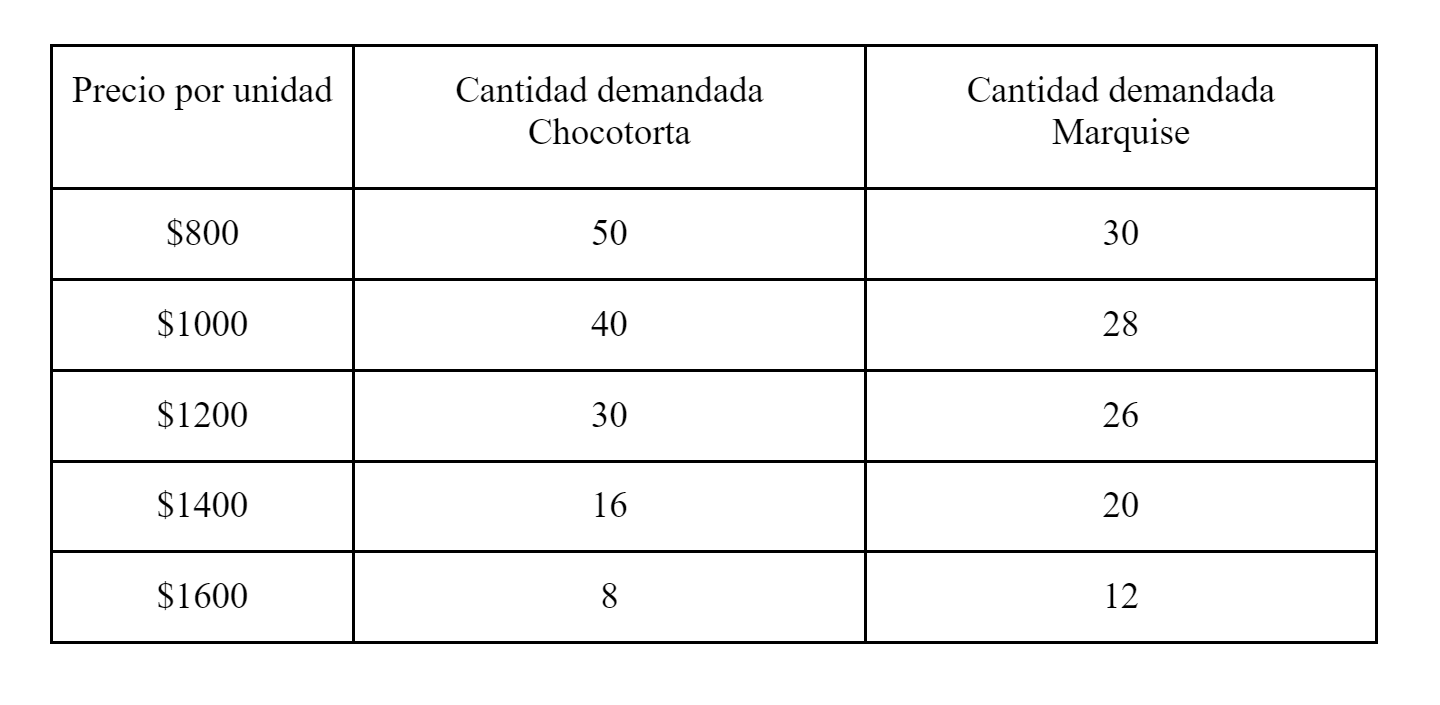
\includegraphics[scale=0.6]{Slides Principios de Economia/Figures/Pachi.png}
\end{frame}

\begin{frame}
\frametitle{El impacto de los impuestos}
\begin{itemize}
    \item ¿Qué es un impuesto?\vspace{2mm}
    \begin{itemize}
        \item Es un tributo generalmente establecido por el Estado 
       \begin{itemize} 
        - para financiar sus gastos
        - para ‘guiar’ el comportamiento (por ejemplo en el caso de externalidades)\vspace{4mm}
        \end{itemize}   
    \end{itemize}
    \item Existen diversos tipos:\vspace{2mm}
    \begin{itemize}
        \item Al consumo, al trabajo, al ingreso, a la propiedad, etc.
    \end{itemize}\vspace{4mm}
    \item Un impuesto aumentará el precio que los consumidores pagan sobre un bien...\vspace{4mm}
    \item La elasticidad precio de la demanda tendrá influencia sobre el efecto del impuesto.
\end{itemize}
\end{frame}

\begin{frame}
\frametitle{Impuestos y eficiencia}
\begin{itemize}
    \item La introducción de impuestos aleja la economía del equilibrio competitivo\vspace{2mm}
    \begin{itemize}
        \item Los impuestos sobre oferentes/consumidores desplazan la curva de oferta/demanda porque el precio es más alto para cada cantidad
        \item Al recaudar impuestos el Estado genera una pérdida de peso muerto.\vspace{4mm}
    \end{itemize}
    \item La recaudación se extrae del excedente de consumidores y productores
    \begin{itemize}
        \item La incidencia del impuesto depende de la elasticidad relativa de consumidores y productores
        \item El grupo menos elástico lleva más de la carga fiscal
    \end{itemize}
\end{itemize}
\end{frame}


\begin{frame}
\frametitle{Impuestos y elasticidad}
\begin{itemize}
    \item Un impuesto puede reducir mucho las ventas si su demanda es altamente elástica.\vspace{2mm}
    \begin{itemize}
        \item ¡Y eso puede ser lo que el gobierno intenta hacer! \\
        - P.ej., impuestos sobre bienes ‘malos’ para la sociedad como el tabaco o el alcohol o por contaminar.\vspace{4mm}
    \end{itemize}
    \item Pero si un impuesto causa una importante caída en las ventas, también reduce los ingresos del impuesto.\vspace{4mm}
    \item Si un gobierno que desea aumentar los ingresos a partir del impuesto, debería elegir gravar productos con demanda inelástica.\vspace{4mm}
    \begin{itemize}
        \item ¿Qué tipo de productos pueden tener una demanda de estas características?
    \end{itemize}
\end{itemize}
\end{frame}

\end{document}

\begin{frame}
\frametitle{Impacto de los impuestos}
\begin{itemize}
    \item ¿Cuánto va a cambiar los impuestos el comportamiento de los individuos?
    \begin{itemize}
        \item ¿Qué tan grande va a ser la pérdida de peso muerto? \\
        - ¿Porqué es relevante conocer la elasticidad de demanda? \\
        - ¿Qué tipo de productos tienen demanda inelástica?
    \end{itemize}
    \item ¿Qué hace el gobierno con los recursos que recauda?
    \item A veces el gobierno quiere cambiar el comportamiento
\end{itemize}
\end{frame}

\begin{frame}
\frametitle{Impacto de un impuesto a los vendedores}
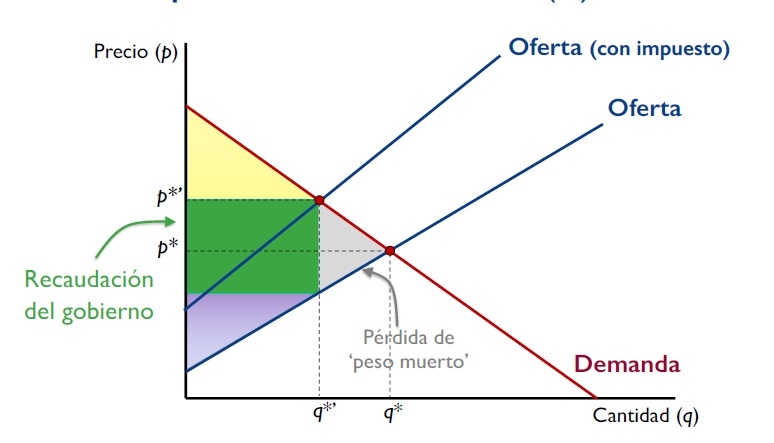
\includegraphics[scale=0.6]{Slides Principios de Economia/Figures/Tema_07.29_impuesto1.jpg}
\end{frame}

\begin{frame}
\frametitle{Impacto de un impuesto a los vendedores}
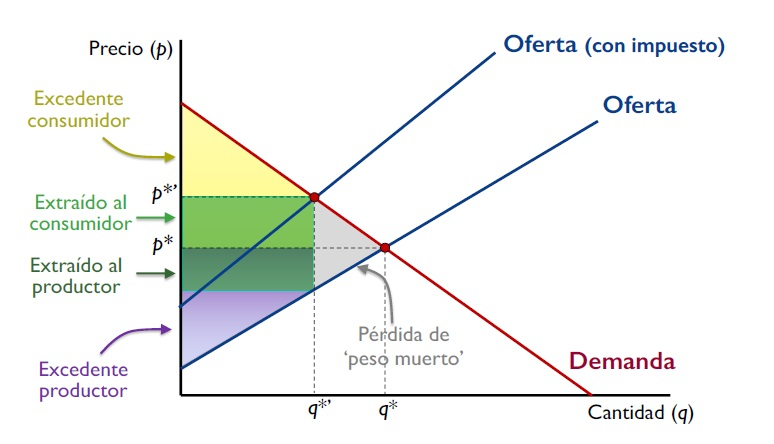
\includegraphics[scale=0.6]{Slides Principios de Economia/Figures/Tema_07.30_impuesto2.jpg}
\end{frame}